% tex/Desenvolvimento/dev_03_arquitetura_modelo.tex
\section{Arquitetura do Modelo: GraphRec Adaptado}
\label{sec:dev_arquitetura_modelo}

\textbf{Definição:} \\
O coração do MatchPredict-AI é uma implementação adaptada da arquitetura **GraphRec** \textcolor{blue}{[\cite{fan2019graphrec}]}, um framework de Redes Neurais em Grafos (GNNs) proposto especificamente para a tarefa de recomendação social. As GNNs são uma classe de redes neurais projetadas para operar diretamente sobre dados estruturados em grafos, permitindo a integração natural de informações dos nós (neste caso, perfis) com a estrutura topológica das conexões entre eles. A implementação do modelo está contida no arquivo `src/models/graphrec.py` e é composta por três módulos principais que interagem para gerar a predição final, conforme ilustrado na Figura \ref{fig:arquitetura_modelo_tcc2}.

\begin{figure}[hbt]
    \centering
    % 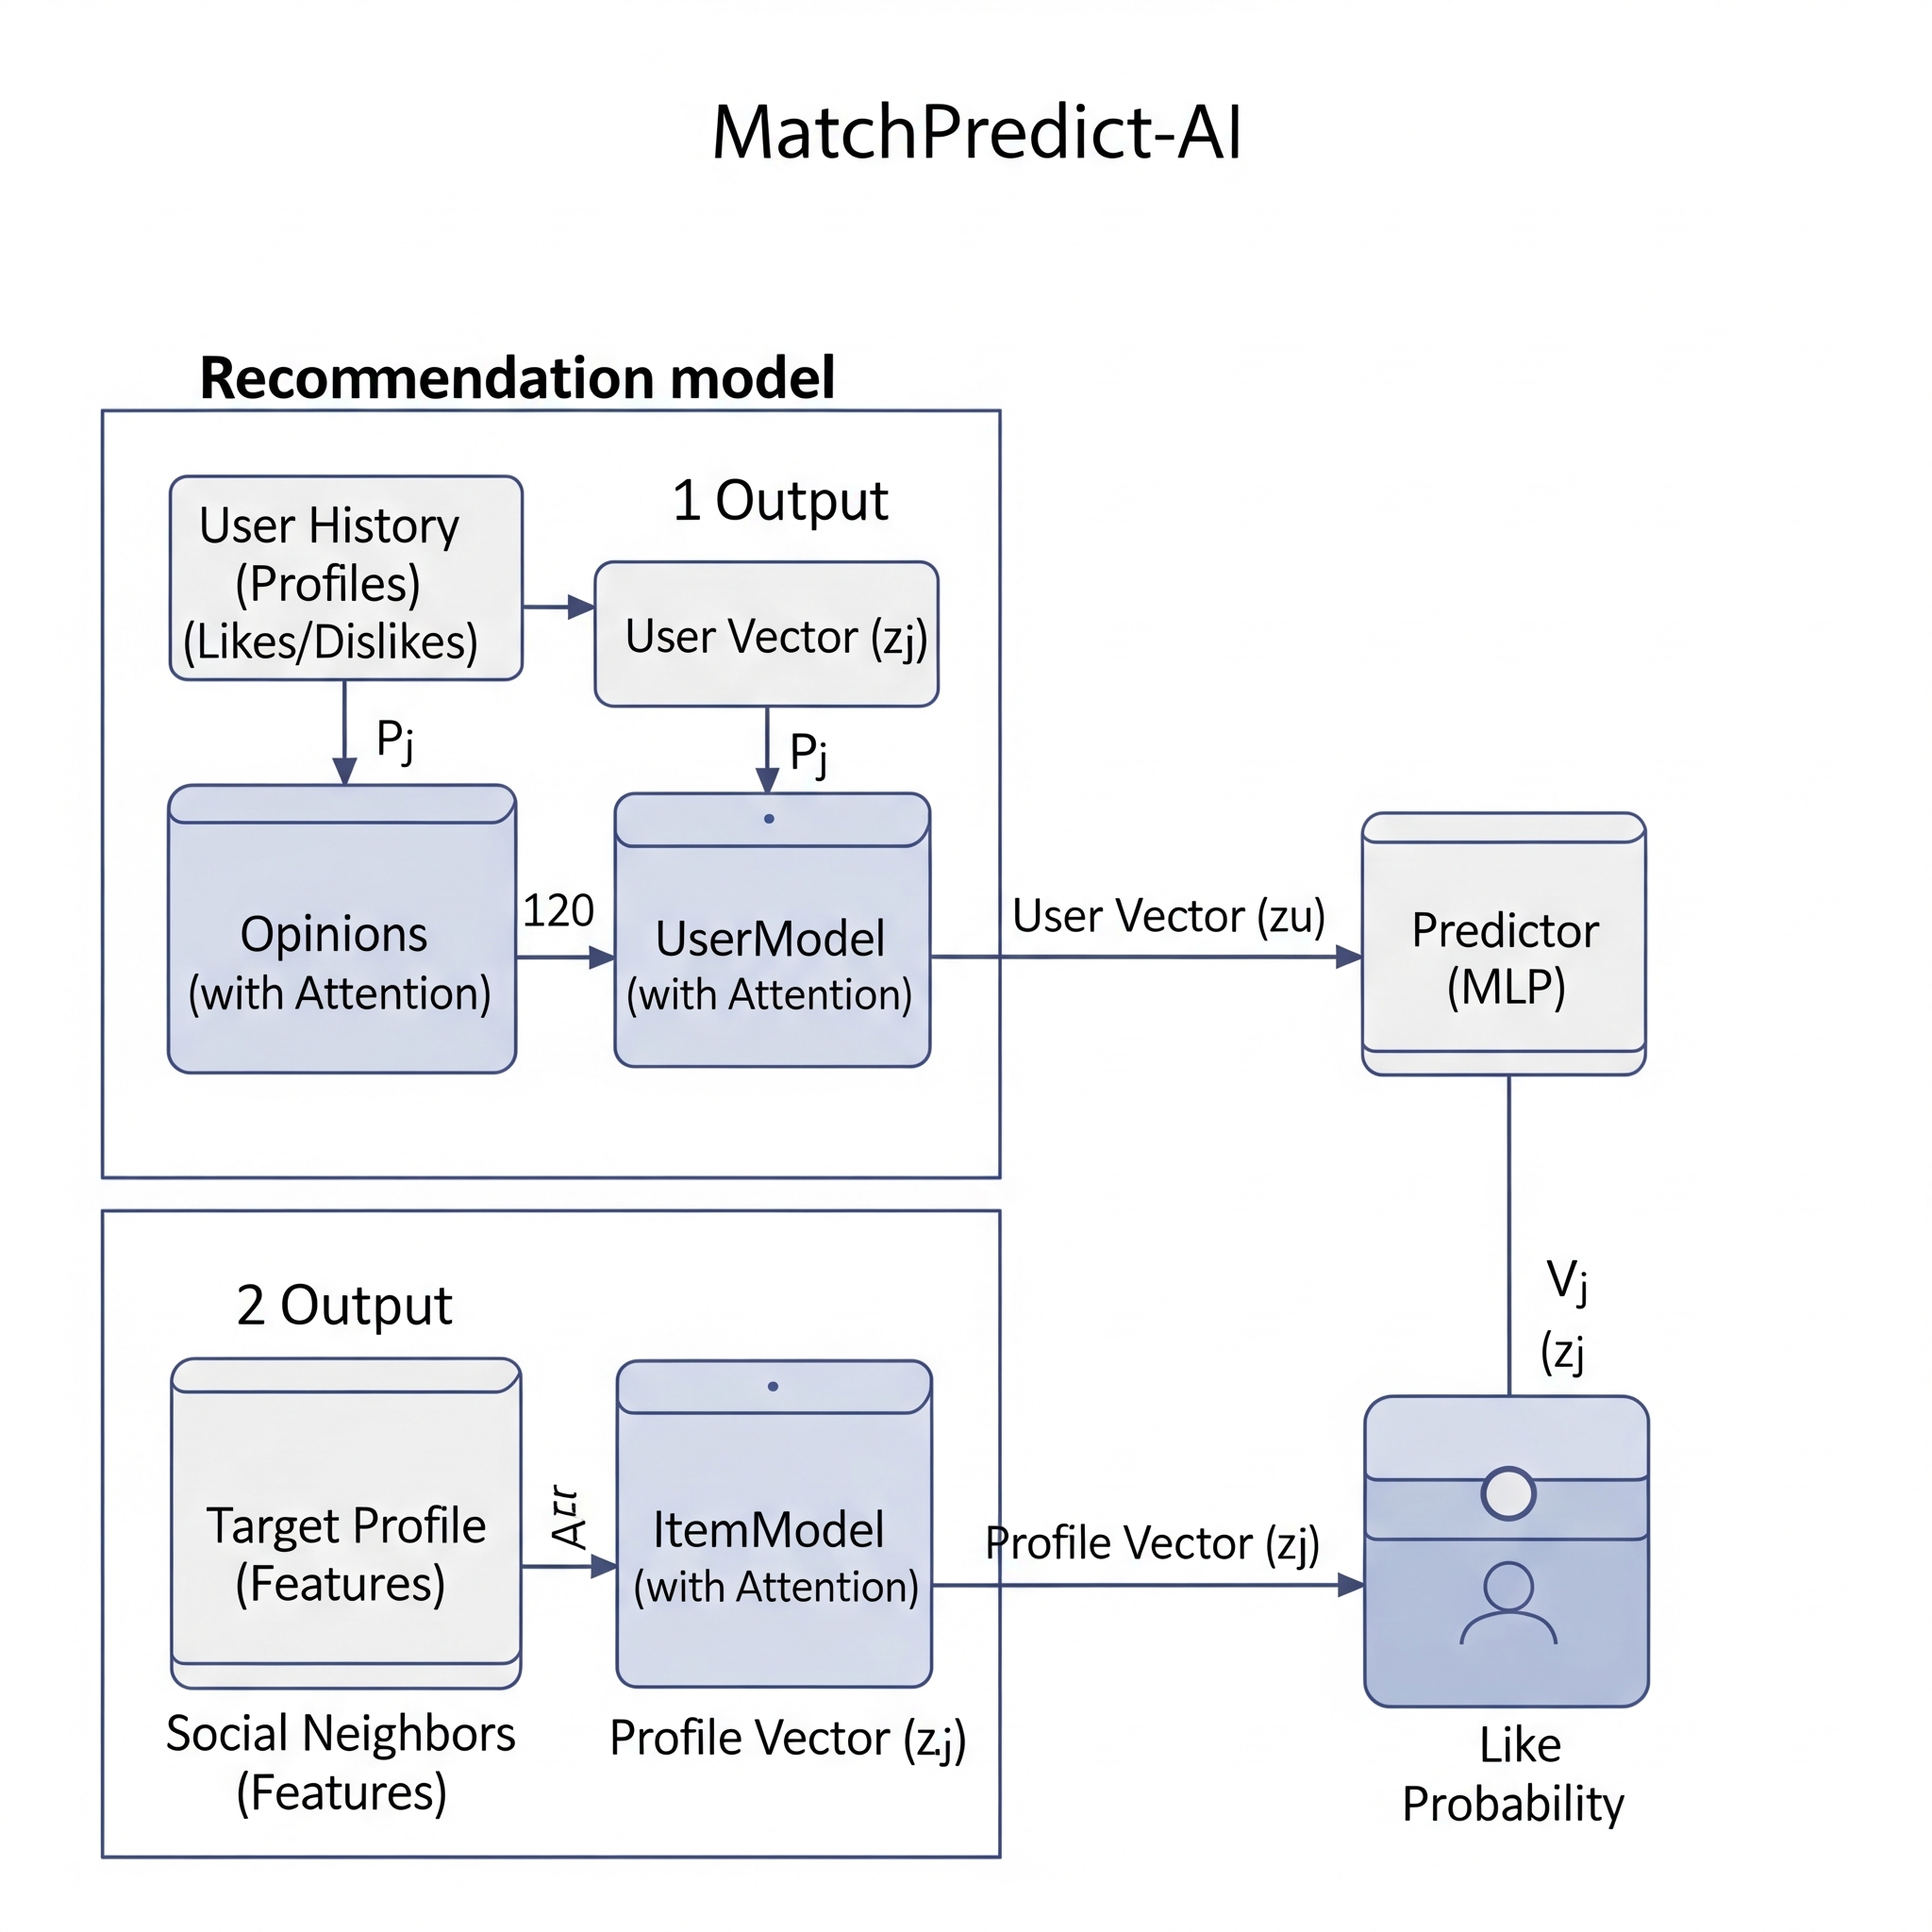
\includegraphics[width=0.8\textwidth]{imagens/diagrama_arquitetura.png} % Lembre-se de criar e adicionar esta imagem
    \framebox[0.9\textwidth][c]{\rule{0pt}{6cm} Espaço para o diagrama da arquitetura do modelo GraphRec}
    \caption{Diagrama da arquitetura do modelo MatchPredict-AI, mostrando a interação entre o UserModel (agregando histórico), o ItemModel (agregando vizinhos sociais) e o Predictor final.}
    \label{fig:arquitetura_modelo_tcc2}
\end{figure}

\textbf{Componentes do Modelo:} \\
A arquitetura do GraphRec implementada é modular e pode ser decomposta nos seguintes componentes:

\begin{itemize}
    \item \textbf{ItemModel:}
    \\ \textbf{Objetivo:} Este módulo é responsável por aprender a representação latente final de um perfil-alvo, denotada como $z_j$. A sua função é enriquecer o vetor de features inicial de um perfil, incorporando o contexto de sua "vizinhança social".
    \\ \textbf{Funcionamento:} Ele recebe como entrada o vetor de 2503 dimensões do perfil-alvo e os vetores correspondentes aos seus 10 vizinhos mais próximos no grafo de similaridade. Através de um **mecanismo de atenção**, o ItemModel aprende a ponderar a importância de cada vizinho. Perfis de vizinhos mais relevantes recebem um peso maior na agregação. As features ponderadas dos vizinhos são então somadas à representação do perfil-alvo. O resultado, $z_j$, é uma representação contextualizada, onde o "significado" de um perfil é influenciado pelos perfis aos quais ele é mais similar.

    \item \textbf{UserModel:}
    \\ \textbf{Objetivo:} Este módulo é projetado para aprender a representação latente do "gosto" de um usuário, denotada como $z_u$. Sua função é capturar as preferências de um usuário a partir de suas interações passadas.
    \\ \textbf{Funcionamento:} A sua entrada é um histórico de perfis com os quais o usuário interagiu (no nosso caso, o histórico simulado pelas personas). O `UserModel` também utiliza um **mecanismo de atenção** para analisar este histórico. Ele aprende a dar pesos diferentes para cada perfil no histórico, permitindo que o modelo foque nos itens mais representativos do gosto do usuário. As features ponderadas dos itens do histórico são então agregadas para formar o vetor final $z_u$, que sintetiza as preferências daquele usuário.

    \item \textbf{Predictor:}
    \\ \textbf{Objetivo:} Este componente final é responsável por realizar a predição de compatibilidade.
    \\ \textbf{Funcionamento:} Trata-se de uma rede neural do tipo Multi-Layer Perceptron (MLP). Ela recebe como entrada a concatenação dos vetores de usuário ($z_u$) e de item ($z_j$) aprendidos pelos módulos anteriores. Através de suas camadas densas com funções de ativação ReLU, o MLP aprende a relação complexa e não-linear entre o gosto de um usuário e as características de um perfil. A camada de saída do MLP produz um único valor (logit), que é então passado por uma função de ativação sigmoide para gerar a probabilidade final de "like", um valor contínuo entre 0 e 1.
\end{itemize}

\textbf{Justificativa da Escolha:} \\
A escolha da arquitetura GraphRec foi motivada por sua capacidade nativa de lidar com os desafios inerentes a dados de recomendação. Ao contrário de modelos mais simples, ela modela conjuntamente as interações e as relações sociais (ou de similaridade), e os mecanismos de atenção permitem que o modelo aprenda de forma diferencial quais vizinhos e quais itens do histórico são mais importantes, refinando significativamente a qualidade da personalização.